%!TEX root = info-main.tex
\section{Performance Evaluation}

We now evaluate the performance of the
proposed detection algorithm via simulation.
We have implemented the proposed {\tt CUBIA} in ns-2
simulator (ver.3.35) \cite{NS2}.

\subsection{Simulation Setup}

%
In the simulation, the multi-AP network is deployed in a $200\times200$
\,$m^2$ area, where 5 APs with 10 client nodes are randomly generated;
this represents a densely-populated configuration fully covering
the entire area.
%
The transmission range and carrier sensing range of legitimate nodes
are set to 75\,m, and 150\,m, respectively. A selfish tethering pair
is placed at the center of the area, whose link distance and carrier
sensing are set to 1\,m and 10\,m, respectively. Table~\ref{table_sim_param}
lists the parameter values used in the simulation study.

\begin{table}[ht]
\renewcommand{\arraystretch}{1.2}
\caption{Parameters used in performance evaluation}
\label{table_sim_param} \centering
\begin{tabular}{|c|c|}
\hline \bfseries Parameter & \bfseries Value \\
\hline
 Transmission range  & 75 \\
 Carrier range       & 150\\
 Data rate / ACK rate & 54\,Mbps / 6\,Mbps \\
 CBR rate per AP-client pair (UDP)& 20\,Mbps \\
 payload size of UDP , TCP& 1000, 1500\,bytes   \\
 $\mathcal{T}_{FER}$ (in Eq.~\eqref{Eq:CUSUMv}) & 0.05 \\
 $\lambda$ (in Eq.~\eqref{Eq:move_avg}) & 0.1\\
 % alex: there is no reference Eq:move_avg
 $m$ & 10\\
 the maximum allowed latency of detection & 2 sec\\
\hline
\end{tabular}
\end{table}

The performance is evaluated in terms of detection accuracy
and time for TCP and UDP protocols. We consider a downlink
scenario where each AP transmits frames to its client nodes.

\begin{figure*} [ht]
\center
  \subfigure[Selfish carrier sensing problem]{  \label{fig-eval-dynamic1}
      \resizebox{55mm}{!}{
      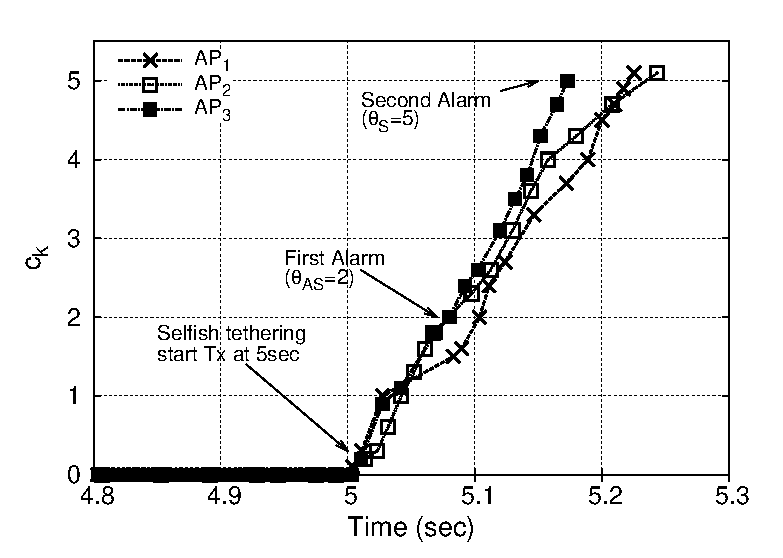
\includegraphics[]{./figures/eval/fig-CUBIA_dynamic-M1_udp}}
      }
  \subfigure[Sudden collisions]{ \label{fig-eval-dynamic2}
      \resizebox{55mm}{!}{
       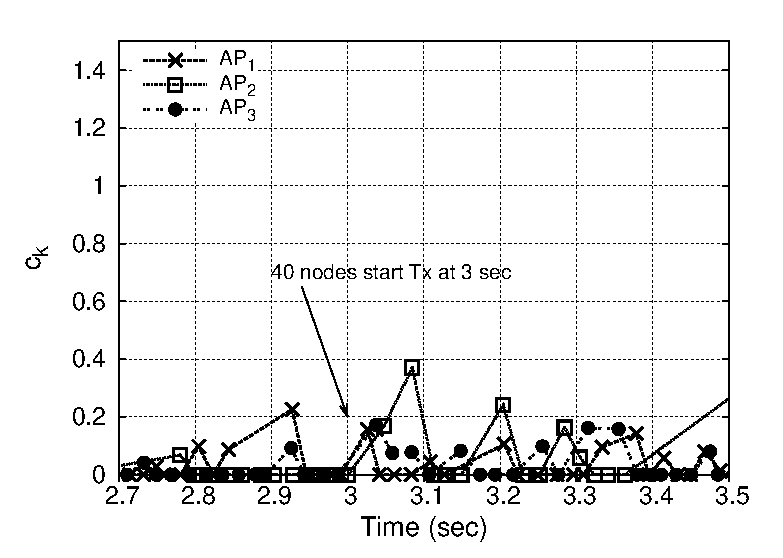
\includegraphics[]{./figures/eval/fig-CUBIA_dynamic-mac}}
       }
       \subfigure[Hidden node problem]{  \label{fig-eval-dynamic3}
\vspace{-0.5cm}
\centering
\epsfxsize=50mm
\epsfbox[50 110 410 402]{./figures/eval/fig-CUBIA_dynamic-hidden}
\vspace{-0.2cm}
      }
\caption{The dynamics of {\tt CUBIA} toward three difference types
of frame losses.}
    \label{fig:eval-differ}
\end{figure*}

\subsection{Detection Performance}

\subsubsection{Accuracy of Frame Loss Differentiation}

To demonstrate the efficacy of {\tt CUBIA} in distinguishing
the selfish carrier sensing problem, we consider three testing
scenarios: (i) selfish carrier sensing, (ii) hidden node problem,
and (iii) collisions.
%
%We first evaluate the effectiveness of the proposed {\tt CUBIA}
%in distinguishing the selfish-carrier-sensing-induced frame losses
%from the other types of frame losses, i.e., hidden node problem
%and collisions.

Fig.~\ref{fig:eval-differ} shows the temporal behavior of CUSUM
change detection filter $c_k$ for the three testing scenarios.
%
Fig.~\ref{fig-eval-dynamic1} plots the results of {\tt CUBIA} over
time for the case of selfish problem in the topology depicted in
Fig.~\ref{fig-patialCH_b}. We can observe that the detection filters
of APs in the interference range continues to increase, where the
selfish node starts transmissions at 5\,s.

Figs.~\ref{fig-eval-dynamic2} and \ref{fig-eval-dynamic3} show
{\tt CUBIA}'s ability of filtering the collisions and the hidden node
problem, respectively.
%
To simulate an abrupt change in the network state, initially,
10 AP--clients pairs are considered until additional 40 nodes
are abruptly activated at 3 second.
%
Fig.~\ref{fig-eval-dynamic2} demonstrates that {\tt CUBIA} effectively
filters out the MAC-layer collisions.
%
To simulate the impact of the hidden node problem, we generated ON/OFF
traffic on a hidden node, as illustrated in Fig.~\ref{fig-eval-dynamic3}.
In the figure, we can see that the detection filter of {\tt CUBIA}
promptly reacts to the hidden node, increasing above $\theta_{AS}$,
but the value of $c_k$ remains low and does not exceed $\theta_{S}$.
%
% alex: it is not clear what do we mean by "adaptive", we need to describe how we adapt RTS/CTS.
This is because the effect of a hidden node is mitigated by adaptive
RTS/CTS changes, thus imparting a negative drift to the detection filter.

Overall, our proposed scheme {\tt CUBIA} accurately distinguishes
the selfish misbehavior with CCA manipulation from collisions and
the hidden node problem.

\subsubsection{Detection Performance}

We now evaluate the detection performance of {\tt CUBIA}.
%
It is important to meet the detectability requirements, such as the
maximum allowed latency of detection. In this simulation study,
we assume that the maximum allowed latency of detection is 2 seconds,
that is, if the selfish misbehavior is not detected within 2 seconds,
we consider this case as a mis-detection.
%
In practice, the detection latency requirement can be adjusted based
on specific needs/conditions of the network and protocol stack.
For example, an extended exposure to selfish carrier sensing can cause
the TCP congestion control and fast recovery algorithms to kick in,
which make it very difficult to recover the throughput performance.
%
There also exists a tradeoff between the detection sensitivity and
the false-alarm rate, which is part of our future work.
%
We run the simulation 150 times for each set of tests with various
backhaul link capacities $B_{cel}$ of selfish tethering, and
alarm thresholds.

Tables~\ref{table:detection-udp} and \ref{table:detection-tcp}
show the detection results for UDP and TCP protocols, respectively.
We can observe that our scheme can detect the selfish behavior with
high backhaul capacity with very high accuracy.
%
Note that $B_{cel}$ implies the intensity of selfish behavior
because the larger the $B_{cel}$, the more outstanding packets the
selfish node can transmit, causing severe interference, as observed
in Section~\ref{sec:channel-selection}.
%
However, the results imply that in many cases, the detection decision
takes more than 2 seconds with low selfish intensity, i.e., small $B_{cel}$.
%
This is because the impact of such a moderately selfish node on the
network performance is not significant, i.e., the selfish node achieves
only a small throughput gain over the legitimate nodes. As a result,
the moderate selfish node is not immediately detectable by {\tt CUBIA}
within 2 seconds, since it takes more samples for the AP to accurately
detect such selfish nodes.
%
Fig.~\ref{fig:throughput-loss} shows the average throughput
degradation ratio of well-behaving nodes due to the selfish node
for various values of selfish intensity (i.e., $B_{cel}$).
The figure implies that a higher selfish intensity incurs
a severer interference on well-behaving nodes.
The throughput degradation can be ignored when the backhaul link
capacity $B_{cel}$ of the selfish node is small.

%%% UDP
\begin{table}[t]\centering
\renewcommand{\arraystretch}{1.2}
\caption{Detection performance for the UDP protocol.}
\label{table:detection-udp}
\setlength{\tabcolsep}{3pt}
\begin{tabular}{c|c|c|c|c}
\hline
%($\theta_{AS}, \theta_{S}$)  & $B_{cel}$={\em 20 Mbps~} & {\em 10 Mbps~} & {\em 5 Mbps~} & {\em 2 Mbps~}\\
\backslashbox{($\theta_{AS}, \theta_{S}$)}{$B_{cel}$} & {\em 20 Mbps~} & {\em 10 Mbps~} & {\em 5 Mbps~} & {\em 2 Mbps~}\\
\hline\hline
(2, 3)&   1.00  & 1.00  & 0.99 & 0.73 \\
(2, 4)&   1.00  & 1.00  & 0.99 & 0.74\\
(2, 5)&   1.00  & 1.00  & 0.97 & 0.61 \\
\hline
(3, 4) &   1.00  & 0.94  & 0.05 & 0.00\\
(3, 5) &   1.00  & 0.93  & 0.07 & 0.00\\
(3, 6) &   0.99  & 0.92  & 0.07 & 0.00\\
\hline
(4, 5) &   1.00  & 0.27  & 0.00 & 0.00\\
(4, 6) &   1.00  & 0.33  & 0.00 & 0.00\\
(4, 7) &   0.95  & 0.27  & 0.00 & 0.00\\
\hline
\end{tabular}	
%\vspace{-0.2cm}
\end{table}

%%% TCP
\begin{table}[t] \centering
\renewcommand{\arraystretch}{1.2}
\caption{Detection performance for the TCP protocol.}
\label{table:detection-tcp}
\setlength{\tabcolsep}{3pt}
\begin{tabular}{c|c|c|c|c}
\hline
\backslashbox{($\theta_{AS}, \theta_{S}$)}{$B_{cel}$} & {\em 20 Mbps~} & {\em 10 Mbps~} & {\em 5 Mbps~} & {\em 2 Mbps~}\\
\hline\hline
(2, 3) &   1.00  & 1.00  & 1.00 & 0.99 \\
(2, 4) &   1.00  & 1.00  & 1.00 & 0.47\\
(2, 5) &   1.00  & 1.00  & 1.00 & 0.03 \\
\hline
(3, 4) &   1.00  & 1.00  & 0.99 & 0.80\\
(3, 5) &   1.00  & 1.00  & 0.98 & 0.28\\
(3, 6) &   1.00  & 1.00  & 0.93 & 0.03\\
\hline
(4, 5) &   0.87  & 0.86  & 0.11 & 0.01\\
(4, 6) &   0.84  & 0.84  & 0.07 & 0.00\\
(4, 7) &   0.63  & 0.72  & 0.02 & 0.00\\
\hline
\end{tabular}	
%\vspace{-0.2cm}
\end{table}


\begin{figure} [ht]
 \center{
        \scalebox{0.55}{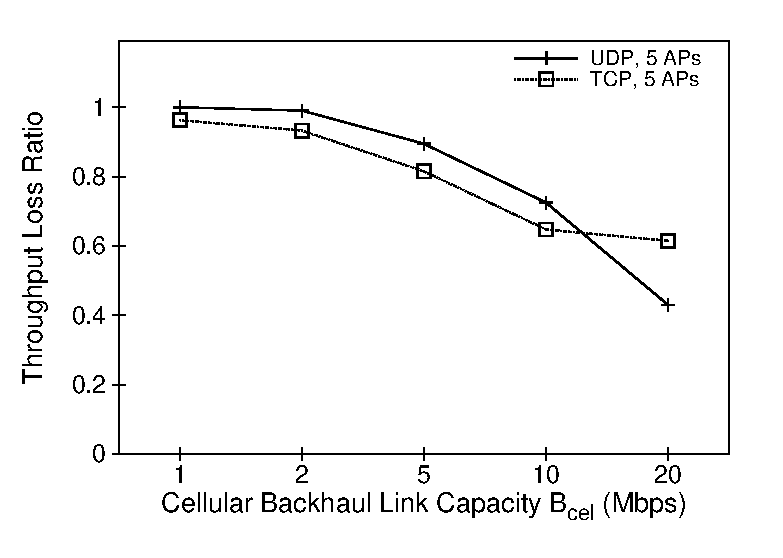
\includegraphics{./figures/eval/sim-sel-loss}}
       }
    \caption{Impact of selfish intensity on the performance of
	well-behaving nodes.}
    \label{fig:throughput-loss}
\end{figure}
%

%\subsubsection{Impact of Design Parameter}

%% Impact of B_{cel}
We next evaluate the impact of the backhaul link capacity $B_{cel}$ of
selfish tethering on the detection performance
for $B_{cel}$ = 2, 5, 10, and 20\! Mbps.
%
Fig.~\ref{fig:impact_bcel} shows the cumulative distribution of detection
time under various $B_{cel}$. The results indicate that more aggressive
selfish behavior, i.e., higher $B_{cel}$, is detected more quickly by
{\tt CUBIA} for both TCP and UDP protocols.
%
This indicates that {\tt CUBIA} can quickly detect aggressive selfish
behaviors, which is a very important design requirement for any good
detection scheme since such an aggressive behavior can seriously
degrade the performance of well-behaving nodes.
%
\begin{figure} [ht]
\center
  \subfigure[UDP]{
      \resizebox{41mm}{!}{
      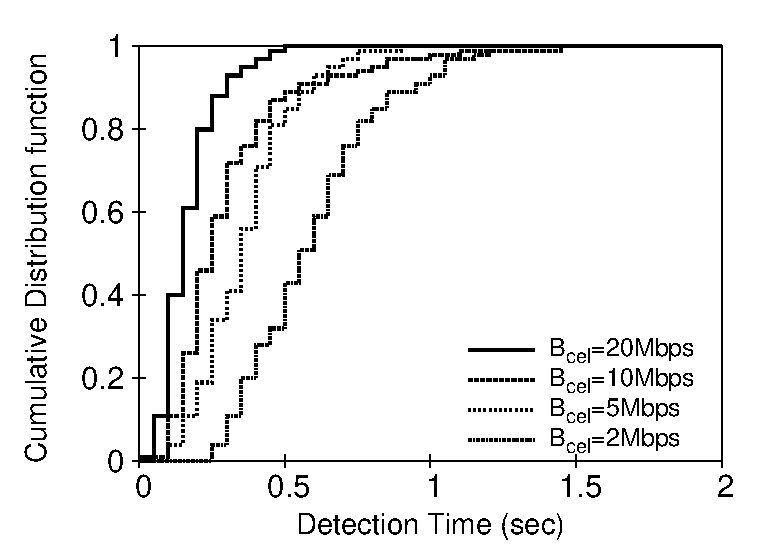
\includegraphics[]{./figures/eval/eval-CDF-detect-udp-M2}}
      }
  \subfigure[TCP]{
      \resizebox{41mm}{!}{
       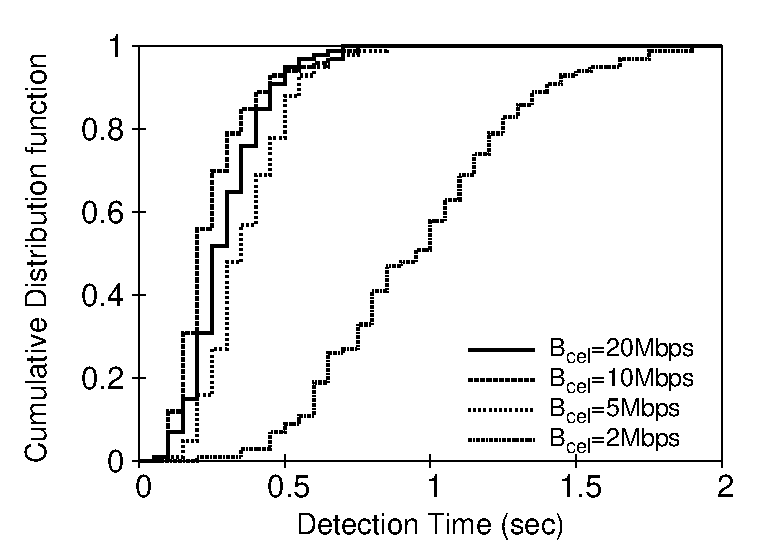
\includegraphics[]{./figures/eval/eval-CDF-detect-tcp-T2}}
       }
    \caption{Impact of $B_{cel}$ on detection time.}
    \label{fig:impact_bcel}
\end{figure}


Finally, we study the impact of alarm thresholds, i.e.,
$\theta_{AS}$ and $\theta_{S}$, on the detection time.
%
Fig.~\ref{fig:impact_threshold1} depicts the distribution of detection time
for 3 different values of the {\em first alarm threshold} $\theta_{AS}$.
%
It is straightforward that the use of a smaller value of $\theta_{AS}$ may
issue the first alarm too frequently and may incur an unnecessary overhead
for RTS/CTS exchange, resulting in the performance degradation. Meanwhile,
the results show that it takes less detection time with
a smaller $\theta_{AS}$.

Similarly, the impact of the {\em second alarm threshold} $\theta_{S}$
can be seen in Fig.~\ref{fig:impact_threshold2}. The figure compares
the detection time for different values of $\theta_{S}$ with
the given $\theta_{AS}$ = 3.
We can see that the detection time increases proportional to $\theta_{S}$.
However, there is a tradeoff between the false alarm ratio and
the detection time according to the choice of $\theta_{S}$.
For example, in case of the temporal behavior of the detection filter in
Fig.~\ref{fig-eval-dynamic3}, the use of a small value of $\theta_{S}$ can
cause false alarms (if $\theta_{S}$ is set to be less than $\theta_{AS}+1$,
it would issue several false alarms.)
although it can reduce the detection time unless the hidden node exists.
Thus, it is recommended to use a value of $\theta_{S}$ larger than
$\theta_{AS}+1$, to avoid false alarms
although it might take more time to detect.
%
\begin{figure} [ht]
\center
  \subfigure[UDP]{
      \resizebox{41mm}{!}{    \label{fig:impact_thresholdAS_UDP}
      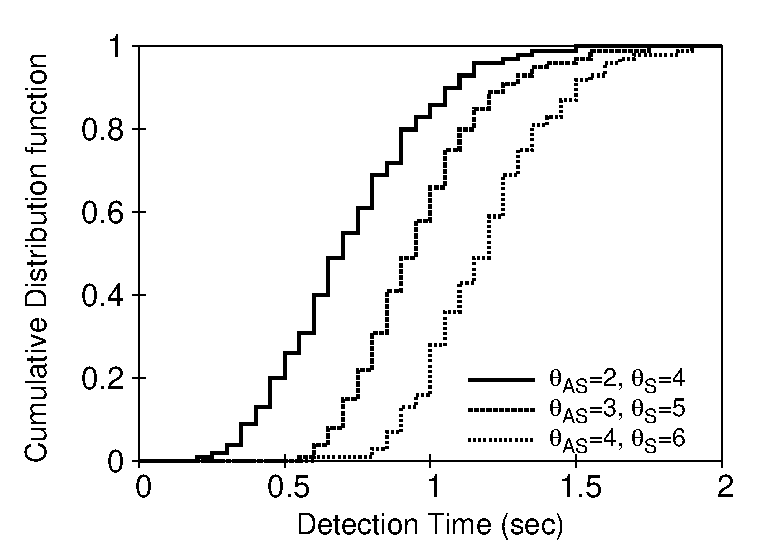
\includegraphics[]{./figures/eval/eval-CDF-impact_Tas-udp}}
      }
  \subfigure[TCP]{
      \resizebox{41mm}{!}{ \label{fig:impact_thresholdAS_TCP}
       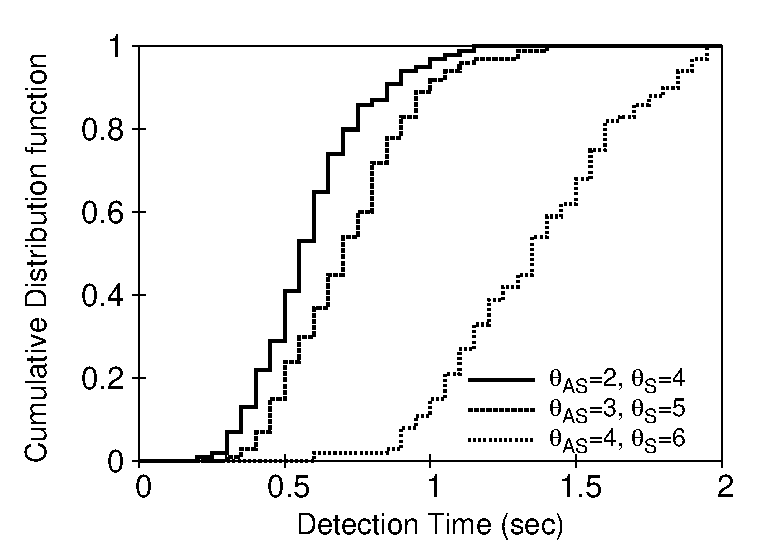
\includegraphics[]{./figures/eval/eval-CDF-impact_Tas-tcp}}
       }
    \caption{Impact of the first alarm threshold $\theta_{AS}$ on detection time
    for UDP and TCP protocols with $B_{cel}$\! =\! 20\! Mbps.}
    \label{fig:impact_threshold1}
\end{figure}
%
%
\begin{figure} [ht]
\center
  \subfigure[UDP]{
      \resizebox{41mm}{!}{    \label{fig:impact_thresholdS_UDP}
      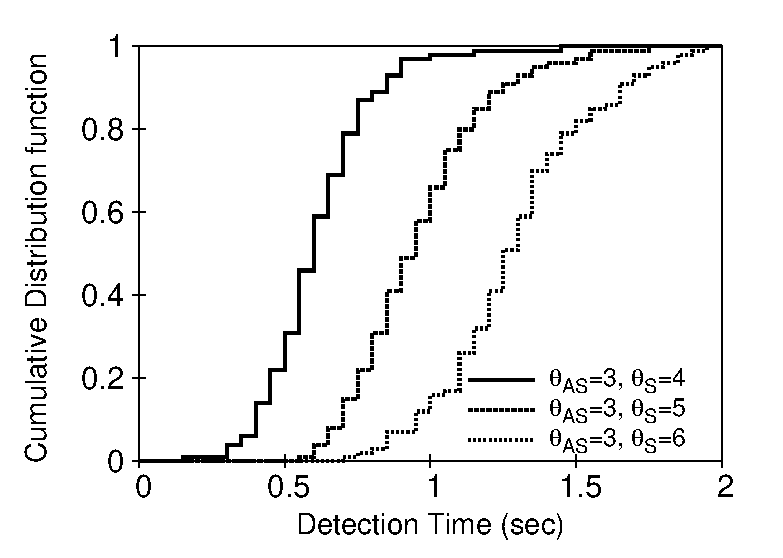
\includegraphics[]{./figures/eval/eval-CDF-impact_dT-udp}}
      }
  \subfigure[TCP]{
      \resizebox{41mm}{!}{ \label{fig:impact_threshold2S_TCP}
       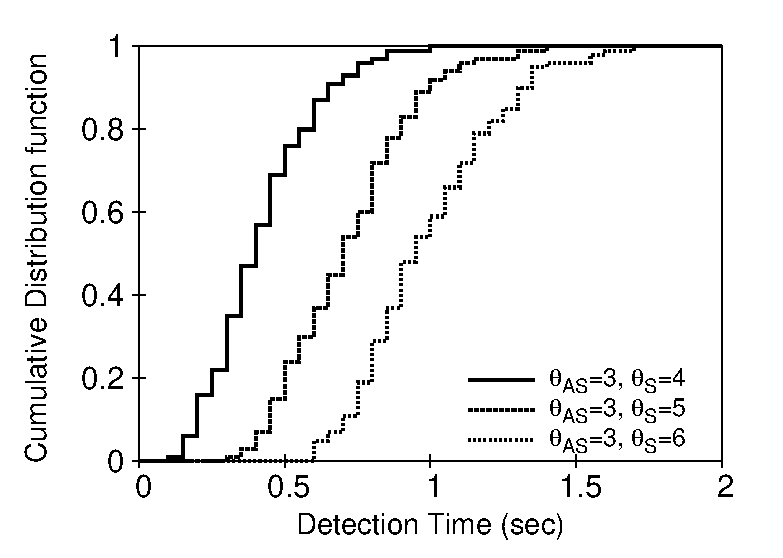
\includegraphics[]{./figures/eval/eval-CDF-impact_dT-tcp}}
       }
    \caption{Impact of the second alarm threshold $\theta_{S}$ for the given $\theta_{AS}$=3
    on detection time with $B_{cel}$\! =\! 20\! Mbps.}
    \label{fig:impact_threshold2}
\end{figure}
